\documentclass{bmvc2k}

%% Enter your paper number here for the review copy
% \bmvcreviewcopy{??}

%\usepackage[brazilian]{babel}
\usepackage[utf8]{inputenc}

\title{Detector e Pintor de Píxeis Similares}

% Enter the paper's authors in order
% \addauthor{Name}{email/homepage}{INSTITUTION_CODE}
\addauthor{Abdullah Zaiter}{abdullah.zaiter@gmail.com}{1}

% Enter the institutions
% \addinstitution{Name\\Address}
\addinstitution{
  Departamento de Ci\^encia da Comptuta\c{c}\~ao\\
  Universidade de Bras\'{\i}lia\\
  Campus Darcy Ribeiro, Asa Norte\\
  Bras\'{\i}lia-DF, CEP 70910-900, Brazil,  
}

\runninghead{Zaiter, Abdullah}{Computer Vision Assignment -- \today}
% Any macro definitions you would like to include
% These are not defined in the style file, because they don't begin
% with \bmva, so they might conflict with the user's own macros.
% The \bmvaOneDot macro adds a full stop unless there is one in the
% text already.
\def\eg{\emph{e.g}\bmvaOneDot}
\def\Eg{\emph{E.g}\bmvaOneDot}
\def\etal{\emph{et al}\bmvaOneDot}

%-------------------------------------------------------------------------
% Document starts here
\begin{document}

\maketitle

\begin{abstract}
    Este documento demonstra os procedimentos, as metodologias e os resultados usados e obtidos no primeiro trabalho da disciplina Princípios de Visão Computacional, o objetivo deste trabalho é obter uma familiarização melhor com a biblioteca OpenCV \cite{opencv_library} por meio da manipulação de imagens ou vídeos levando em consideração o pixel clicado pelo usuário.
\end{abstract}

%-------------------------------------------------------------------------
\section{Introdução}
\label{sec:intro}
    Há varias representações digitais de uma imagem, por exemplo, para uma imagem em preto e branco, o comum é que a imagem seja representada na forma de uma matriz de profundidade 1, onde cada píxel é de uma dimensão e um valor, geralmente entre 0 e 255, enquanto a representação mais comum de imagens coloridas é RGB, nesta representação a matriz tem profundidade 3 onde cada píxel possui 3 valores, cada um representa o valor da intensidade de cada cor, das 3 cores, azul, verde e vermelho que geralmente também variam entre 0 e 255. Considerando isso, para que seja possível a identificação quais píxeis são mais similares sem depender da profundidade da imagem (espaço de cor) , pode-se usar a equação de distancia euclidiana:
    \begin{equation}\label{eq:geneuc}
        d = \sqrt{(x_2 - x_1)^2 + (y_2 - y_1)^2 + (z_2 - z_1)^2...}
    \end{equation} 
    Para o caso do espaço de cor Grayscale (profundidade 1) a equação torna-se:
    \begin{equation}\label{eq:gen1d}
        d = \sqrt{(G_2 - G_1)^2}
    \end{equation}
    \vspace{-3mm}
    \begin{equation}\label{eq:1dsimp}
        d =\hspace{2mm} \mid(G_2 - G_1)\mid
    \end{equation}
    \vspace{1mm}
    Enquanto para o caso de RGB (profundidade 3) a equação é:
    \begin{equation}\label{eq:rgbeucgen}
        d = \sqrt{(B_2 - B_1)^2 + (G_2 - G_1)^2 + (R_2 - R_1)^2}
    \end{equation}
    \vspace{-3mm}
    \begin{equation}\label{eq:rgbeuc}
        d^2 = (B_2 - B_1)^2 + (G_2 - G_1)^2 + (R_2 - R_1)^2
    \end{equation}
    Para fazer este trabalho, foi usada a biblioteca \textit{OpenCV} em \textit{Python}. O \textit{OpenCV} é uma biblioteca de funções de programação voltada principalmente para a visão computacional em tempo real. Originalmente desenvolvido pela Intel, foi posteriormente apoiado pela \textit{Willow Garage} e pela \textit{Itseez}, e em 2016 a \textit{Intel} comprou a \textit{Itseez} e em consequência a biblioteca. \textit{OpenCV} é multiplataforma e gratuita para uso sob a licença \textit{BSD} de código aberto.
\section{Metodologia}
    Para melhor controle de versão e rastreamento de mudanças, foi utilizada a ferramenta Git em um  \href{https://github.com/abdullah-zaiter/Similar-Pixels-Detector}{Repositório} do autor no site \href{https://github.com}{GitHub}.\\
    Sendo aluno de Engenharia Mecatrônica e vindo da areá de robótica e sistemas embarcados, a eficiência e velocidade  do programa sem a alta utilização de recursos computacionais, são características de extrema importância e as mesmas foram levadas em conta no desenvolvimento do código, fazendo com que o código seja compacto e de eficiência alta. \\
    A captura do clique do usuário na imagem era rastreado pela função \textit{mouseCallback} \cite{MouseCallback}.\\
    O trabalho foi dividido em quatro etapas, que são basicamente os requisitos demandados:
    \begin{itemize}
        \item \textbf{Etapa 1:} Abrir um arquivo de imagem \cite{imgread} (do tipo JPG) e permitir ao usuário clicar com o botão esquerdo do mouse sobre um ponto na área da imagem e mostrar no terminal a coordenada do ponto \textit{(row,column)} na imagem, informando os valores do pixel RGB, quando a imagem for colorida ou o valor da intensidade do pixel quando a imagem for em nível de cinza \textit{(greyscale)}.
        \item \textbf{Etapa 2:} Criar uma rotina de seleção de píxeis baseado na cor de onde for clicado, comparar o valor da cor (ou tom de cinza) de todos os píxeis da imagem com o valor da cor (ou tom de cinza) de onde foi clicado. 
        Se a diferença entre esses valores for menor que 13, marcar o pixel com a cor vermelha e exiba o resultado na tela.
        \item \textbf{Etapa 3:} Abrir um arquivo de vídeo (padrão avi ou x264) e realizar os mesmos procedimentos da etapa 2 durante toda a execução do vídeo. Cada vez que o usuário clica na imagem, o valor de referência deve ser atualizado.
        \item \textbf{Etapa 4:} Abrir o \textit{streaming} de vídeo de uma \textit{webcam} ou câmera USB conectada ao computador e realize todos os procedimentos solicitados na etapa 3.
    \end{itemize}
    O desempenho alto atingido pelo código foi devido a Não usar laços \textit{for} e \textit{while} no código (tirando o lanço principal do programa) fazendo todas as operações necessarias por meio de operações matriciais da biblioteca \textit{Numpy} \cite{noloop} e operações lógicas (\textit{Bitwise}).\\
    O algoritmo da lógico consiste em 3 funções base:
    \begin{itemize}
        \item \textbf{isImageInGrayScale(image)}: Esta função recebe uma imagem como parâmetro e retorna Verdadeiro caso a imagem for em Grayscale e Falso caso contrário.\\
        Isto é determinado pelo fato que em fotos grayscale os canais RGB possuem o mesmo valor, assim, os canais RGB da imagem recebida são separados usando a função \textit{Split} \cite{splitshapemerge}, após isso, é checada a diferença entre esses canais, se não for zero, esta imagem não é em Grayscale \cite{colorspaces}.
        \item \textbf{distanceMatCalculator(pixel,image, read\_mode)}: Esta função recebe uma imagem qualquer e um valor referencia do pixel clicado pelo usuário e o modo de leitura da imagem (grayscale ou RGB) e retorna uma imagem binarizada indicado os píxeis que serão pintados.\\ 
        Isto é feito criando uma imagem auxiliar com a cor do pixel clicado igual ao tamanho da imagem original, faz a subtração entre as duas imagens, pro caso do Grayscale, este valor já é o suficiente (pela equação \ref{eq:1dsimp}) para gerar a matriz a ser retornada \cite{MatForImage}. Pro caso de RGB, após a mesma subtração, os canais da imagem são usados para calcular a distancia euclidiana pela equação \ref{eq:rgbeuc}, pois assim não necessário o uso da função raíz que tem um custo computacional mais alto, assim a distancia ao quadrado é a métrica de decisão. Para gerar uma imagem binarizada a partir de uma matriz de distancias, foi utilizada a função \textit{threshold} do \textit{OpenCV} \cite{threshold} por fazer isto mais rápido que método de iteração feito manualmente por loops em \textit{Python}.
        \item \textbf{insertRedByBinary(binary\_img, image, read\_mode)}:Esta função recebe a imagem binarizada, a imagem original e o modo de leitura da imagem (grayscale ou RGB) e retorna a imagem pintada de vermelho nos locais indicados pela imagem binarizada.
        Primeiramente, converte a imagen original para RGB caso estiver em Grayscale, após isso, separa os canais RGB da imagem e faz as operações lógicas a seguir :
        \[R = binary\_img ~|~ R\]
        \vspace{-3mm}
        \[binary\_img =~ \sim (binary\_img)\]
        \vspace{-3mm}
        \[B = binary\_img ~\&~ B\]
        \vspace{-3mm}
        \[G = binary\_img ~\&~ G\]
        Após isso, é usada a função \textit{merge} \cite{splitshapemerge} do \textit{OpenCV} para gerar a imagem resultante, a partir dos canais RGB manipulados, pintada de vermelho nos píxeis adequados.
    \end{itemize}
    Além disso, ao invés de ter 4 códigos na entrega, referentes a cada requisito do trabalho, foi decidido gerar somente um código que atenda todos os requisitos por meio de interface com o usuário, mostrada no fluxograma da Figura~\ref{fig:fluxograma}.
    \begin{figure}[!ht]
        \centering
        %\captionsetup{justification=centering}
        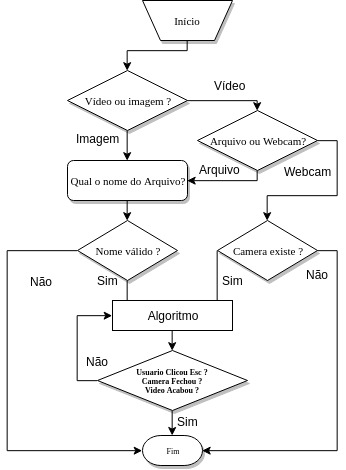
\includegraphics[scale=.55]{Figs/flowchart.jpg}
        \vspace{-3mm}
        \caption{Fluxograma do código}
        \label{fig:fluxograma}
    \end{figure}
    \begin{figure}[!ht]
        \centering
        %\captionsetup{justification=centering}
        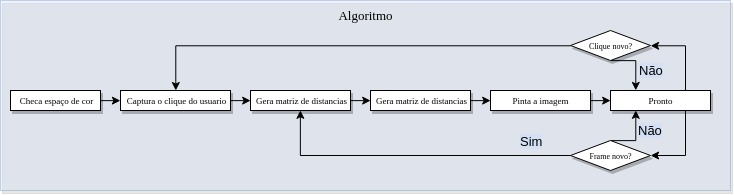
\includegraphics[scale=.45]{Figs/algoritmo.jpg}
        \vspace{-3mm}
        \caption{Etapas do algoritmo}
        \label{fig:fluxograma}
    \end{figure}
\newpage
\section{Resultados}
    Após o desenvolvimento do código, foram coletados os dados a seguir:
    \begin{itemize}
        \item  Etapa 1:
            \begin{figure}[!ht]
                \centering
                %\captionsetup{justification=centering}
                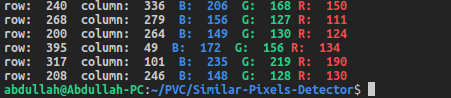
\includegraphics[scale=.60]{Figs/printpixrgb.png}
                \vspace{-3mm}
                \caption{Valores do píxel RGB clicado e a posição do mesmo}
                \label{fig:terminalrgb}
            \end{figure}
            \begin{figure}[!ht]
                \centering
                %\captionsetup{justification=centering}
                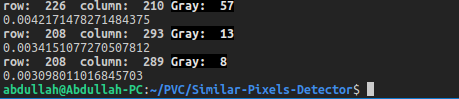
\includegraphics[scale=.60]{Figs/printpixgray.png}
                \vspace{-3mm}
                \caption{Valores do píxel Grayscale clicado e a posição do mesmo}
                \label{fig:terminalgray}
            \end{figure}
        \item Etapa 2:
            \begin{figure}[!ht]
                \centering
                %\captionsetup{justification=centering}
                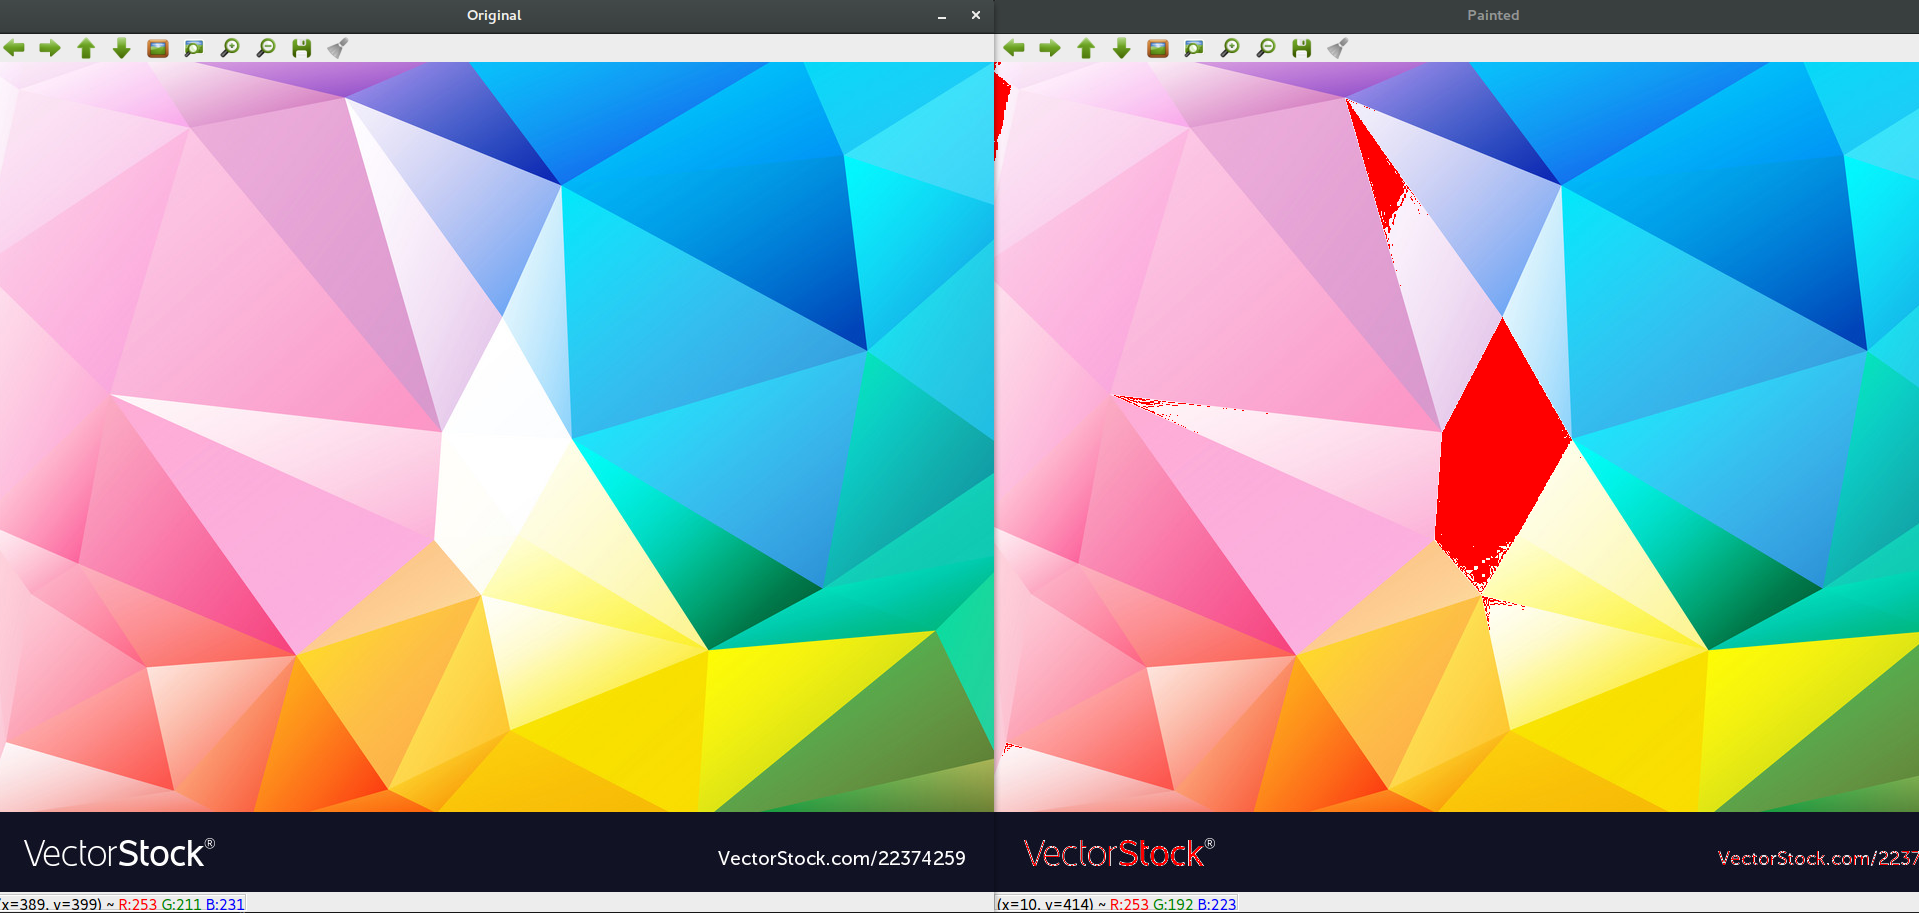
\includegraphics[scale=.16]{Figs/coloreddemonst.png}
                \vspace{-3mm}
                \caption{Funcionamento com imagem RGB}
                \label{fig:rgbpainted}
            \end{figure}
            \begin{figure}[!ht]
                \centering
                %\captionsetup{justification=centering}
                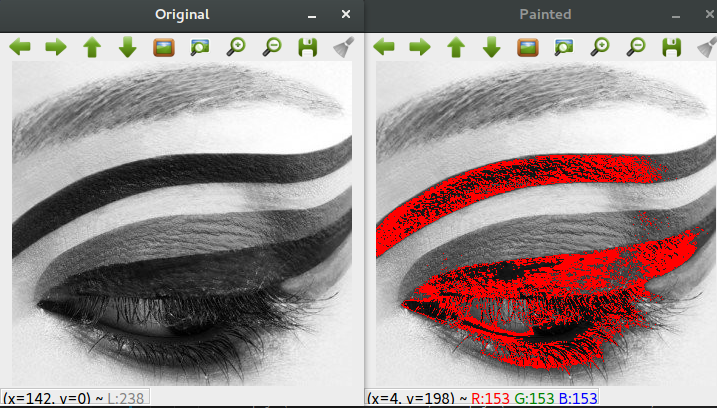
\includegraphics[scale=.315]{Figs/grayscaledemonst.png}
                \vspace{-3mm}
                \caption{Funcionamento com imagem Grayscale}
                \vspace{-7mm}
                \label{fig:graypainted}
            \end{figure}
        \item Etapa 3:\\
            \vspace{-5mm}
            \begin{figure}[!ht]
                \centering
                %\captionsetup{justification=centering}
                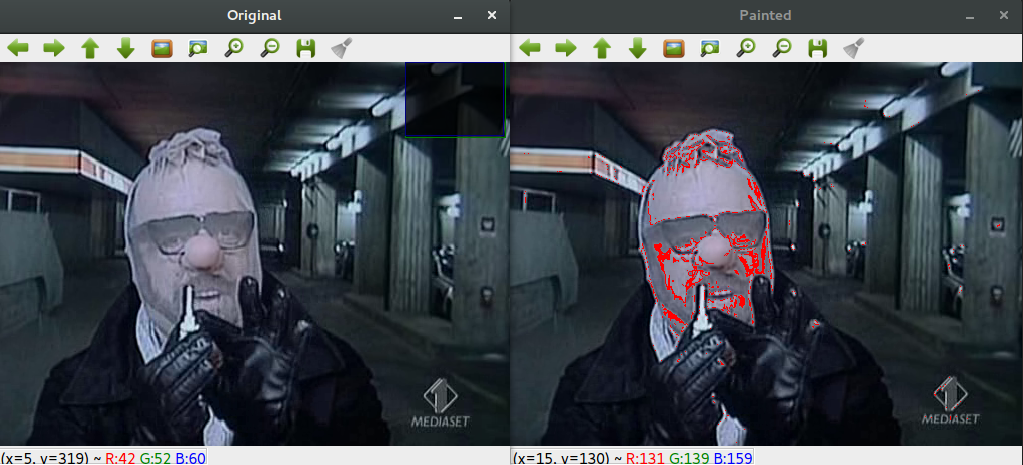
\includegraphics[scale=.33]{Figs/video_test.png}
                \vspace{-3mm}
                \caption{Funcionamento com video .avi}
                \vspace{-7mm}
                \label{fig:videotest}
            \end{figure}
        \item Etapa 4:
            \vspace{-2mm}
            \begin{figure}[!ht]
                \centering
                %\captionsetup{justification=centering}
                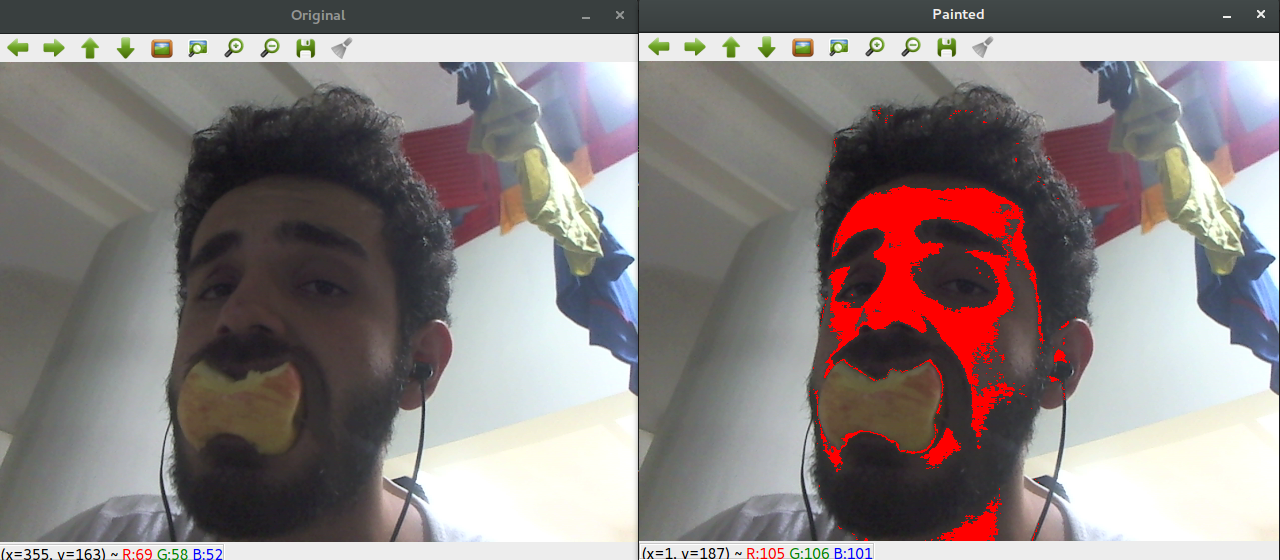
\includegraphics[scale=.26]{Figs/webcamtest.png}
                \vspace{-3mm}
                \caption{Funcionamento com webcam}
                \vspace{-7mm}
                \label{fig:webcamtest}
            \end{figure}
        \item Geral:
            \vspace{-1mm}
            \begin{table}[!ht]
                \centering
                \begin{tabular}{|c|c|c|c|}
                    \hline
                    \textbf{Resolução (WxH)} & 340x325 (Grayscale) & 512x512 (RGB) & 1000x830 (RGB)  \\ \hline
                    \textbf{Tempo (s)}       &    0.0035     &    0.0163     &      0.0452     \\ \hline
                \end{tabular}
                \vspace{2mm}
                \caption{Media de tempo de processamento calculada usando 5 valores de cliques diferentes}
                \label{tab:eficiencia}
            \end{table}
    \end{itemize}
\newpage
\section{Discussão e Conclusões}
    Foi possível a realização e a validação de todos os requisitos do trabalho, os resultados foram satisfatórios e condizentes, serão discutidos para cada requisito respectivamente a seguir:
    \begin{itemize}
        \item \textbf{Requisito 1}\\
            Como pode ser visto nas Figuras \ref{fig:terminalrgb} e \ref{fig:terminalgray}, usando a função \textit{mouseCallBack} do \textit{OpenCV} e técnicas de colorir \textit{strings} no terminal, foi possível rastrear o clique do usuário e mostrar no terminal a posição clicada com o respectivo valor do píxel.
        \item \textbf{Requisito 2}\\
            Nas Figuras \ref{fig:rgbpainted} e \ref{fig:graypainted} encontram se a direita a imagem original e a esquerda a imagem com o algoritmo aplicado demonstrando o funcionamento, o resultado foi condizente. Foi notado que o desempenho do algoritmo é melhor com imagens no espaço de cor Grayscale do que com imagens no espaço de cor RGB devido a simplificação adotada para equação da distancia euclidiana no caso de uma dimensão, demonstrada na equação \ref{eq:gen1d}.
        \item \textbf{Requisito 3}\\
            Foi testado o algoritmo com vários vídeos de resoluções e durações diferentes, e foi medida a eficiência do mesmo nestes vídeos, a partir dos tempos de processamento por frame calculados na Tabela \ref{tab:eficiencia}, foi obtida a tabela a seguir
            \begin{table}[!ht]
                \centering
                \begin{tabular}{|c|c|c|c|}
                    \hline
                    \textbf{Resolução (WxH)} & 340x325 (Grayscale) & 512x512 (RGB) & 1000x830 (RGB)  \\ \hline
                    \textbf{FPS}       &    285     &    62     &      22     \\ \hline
                \end{tabular}
                \vspace{2mm}
                \caption{FPS calculados}
                \label{tab:fps}
            \end{table}
            Sendo que os testes foram realizados em uma maquina com o processador Intel Celeron N3450, que é um processador inferior, em outros processadores melhores o desempenho será superior.
        \item \textbf{Requisito 4}\\
            O teste da \textit{Webcam} foi feito com uma camera Logitech HD 1080p, o algoritmo agiu no video e implicou em nenhum travamento visível.
    \end{itemize}


\newpage
\bibliography{refs}
\end{document}